%% PNAStwoS.tex
%% Sample file to use for PNAS articles prepared in LaTeX
%% For two column PNAS articles
%% Version1: Apr 15, 2008
%% Version2: Oct 04, 2013

%% BASIC CLASS FILE
\documentclass{pnastwo}

%% ADDITIONAL OPTIONAL STYLE FILES Font specification

%\usepackage{pnastwoF}



%% OPTIONAL MACRO DEFINITIONS
\def\s{\sigma}
%%%%%%%%%%%%
%% For PNAS Only:
\url{www.pnas.org/cgi/doi/10.1073/pnas.0709640104}
\copyrightyear{2008}
\issuedate{Issue Date}
\volume{Volume}
\issuenumber{Issue Number}
%\setcounter{page}{2687} %Set page number here if desired
%%%%%%%%%%%%

\begin{document}

\title{Friction at Water / Ice-I$_\mathrm{h}$ interfaces: Do the
  Different Facets of Ice Have Different Hydrophilicity?}

\author{Patrick B. Louden
\and
J. Daniel Gezelter\affil{1}{Department of Chemistry and Biochemistry, University of Notre Dame, Notre Dame,
IN 46556}}

\contributor{Submitted to Proceedings of the National Academy of Sciences
of the United States of America}

%%%Newly updated.
%%% If significance statement need, then can use the below command otherwise just delete it.
\significancetext{RJSM and ACAC developed the concept of the study. RJSM conducted the analysis, data interpretation and drafted the manuscript. AGB contributed to the development of the statistical methods, data interpretation and drafting of the manuscript.}

\maketitle

\begin{article}
\begin{abstract}
{In this follow up paper of the basal and prismatic facets of the 
Ice-I$_\mathrm{h}$/water interface, we present the 
pyramidal and secondary prismatic 
interfaces for both the quiescent and sheared systems. The structural and
dynamic interfacial widths for all four crystal facets were found to be in good
agreement, and were found to be independent of the shear rate over the shear 
rates investigated. 
Decomposition of the molecular orientational time correlation function showed
different behavior for the short- and longer-time decay components approaching
normal to the interface. Lastly we show through calculation of the interfacial
friction coefficient that the basal and pyramidal facets are more 
hydrophilic than the prismatic and secondary prismatic facets.}
\end{abstract}

\keywords{ice|water|interface|contact angle|molecular dynamics}

\abbreviations{QLL, quasi liquid layer; MD, molecular dynamics}

%\dropcap{I}n this article we study the evolution of ``almost-sharp'' fronts
%for the surface quasi-geostrophic equation. This 2-D active scalar
%equation reads for the surface quasi-geostrophic equation.
%\begin{equation}
%\mfrac{D \theta}{Dt}=\mfrac{\pr \theta}{\pr t} + u\cdot \nabla
%\theta=0 \label{qg1}
%\end{equation}

The Ice-I$_\mathrm{h}$/water quiescent interface has been extensively studied 
over the past 30 years by theory and experiment. Haymet \emph{et al.} have 
done significant work characterizing and quantifying the width of these 
interfaces for the SPC,\cite{Karim90} SPC/E,\cite{Gay02,Bryk02}, 
CF1,\cite{Hayward01,Hayward02} and TIP4P\cite{Karim88} models for water.\cite{Bryk04,Smith05,Wilson08,Wilson10} Nada and Furukawa have studied
the the basal- and prismatic-water interface width\cite{Nada95} and crystal 
surface restructuring at temperatures approaching the melting 
point\cite{Nada00}.

It is well known that the surface of ice exhibits a premelting layer at 
temperatures near the melting point, often called a quasi-liquid layer (QLL).
Molecular dynamics simulations of the facets of ice-I$_\mathrm{h}$ exposed
to vacuum performed by Conde, Vega and Patrykiejew have found QLL widths of
approximately 10 \AA\ at 3 K below the melting point\cite{Conde08}.
Similarly, Limmer and Chandler have used course grain simulations and 
statistical field theory to estimated QLL widths at the same temperature to
be about 3 nm\cite{Limmer14}.
Recently, Sazaki and Furukawa have developed an experimental technique with 
sufficient spatial and temporal resolution to visulaize and quantitatively
analyze QLLs on ice crystals at temperatures near melting\cite{Sazaki10}. They 
have found the width of the QLLs perpindicular to the surface  at -2.2$^{o}$C 
to be 3-4 \AA\ wide. They have also seen the formation of two immiscible
QLLs, which displayed different stabilities and dynamics on the crystal 
surface\cite{Sazaki12}. 

There is significant interest in the properties of ice/ice and ice/water 
interfaces in the geophysics community. Most commonly, the results of shearing
two ice blocks past one 
another\cite{Casassa91, Sukhorukov13, Pritchard12, Lishman13} or the shearing 
of ice through water\cite{Cuffey99, Bell08}. Using molecular dynamics 
simulations, Samadashvili has recently shown that when two smooth ice slabs 
slide past one another, a stable liquid-like layer develops between 
them\cite{Samadashvili13}. To fundamentally understand these processes, a 
molecular understanding of the ice/water interfaces is needed.     
Investigation of the ice/water interface is also crucial in understanding
processes such as nucleation, crystal 
growth,\cite{Han92, Granasy95, Vanfleet95} and crystal 
melting\cite{Weber83, Han92, Sakai96, Sakai96B}. 
  
In a previous study\cite{Louden13}, we investigated
the basal and prismatic facets of an ice-I$_\mathrm{h}$/water
interface where the ice was sheared relative to the liquid. Using
 velocity shearing and scaling approach to reverse 
non-equilibrium molecular dynamics (VSS-RNEMD), simultaneous temperature and 
velocity gradients were applied to the system, allowing for measurment
of friction and thermal transport properties while maintaining a stable 
interfacial temperature\cite{Kuang12}. 

Paragraph here about hydrophobicity and hydrophilicity, maybe move up
more in the paper as well. Talk about physically what it means for a 
surface to by hydrophobic or hydrophilic, and then we move into
how do we define it (mathematically) and then measure the degree
of wetting experimentally and theoretically.

The hydrophobicity or hydrophilicity of a surface can be described by the
extent a droplet of water wets the surface. The contact angle formed between
the solid and the liquid, $\theta$, which relates the free energies of the 
three interfaces involved, is given by Young's equation.
\begin{equation}\label{young}
\cos\theta = (\gamma_{sv} - \gamma_{sl})/\gamma_{lv}
\end{equation} 
Here $\gamma_{sv}$, $\gamma_{sl}$, and $\gamma_{lv}$ are the free energies
of the solid/vapor, solid/liquid, and liquid/vapor interfaces respectively.
Large contact angles ($\theta$ $\gg$ 90\textsuperscript{o}) correspond to low 
wettability and hydrophobic surfaces, while small contact angles 
($\theta$ $\ll$ 90\textsuperscript{o}) correspond to high wettability and 
hydrophilic surfaces. Experimentally, measurements of the contact angle
of sessile drops has been used to quantify the extent of wetting on surfaces
with thermally selective wetting charactaristics\cite{Tadanaga00,Liu04,Sun04},
as well as nano-pillared surfaces with electrically tunable Cassie-Baxter and 
Wenzel states\cite{Herbertson06,Dhindsa06,Verplanck07,Ahuja08,Manukyan11}. 
Luzar and coworkers have done significant work modeling these transitions on 
nano-patterned surfaces\cite{Daub07,Daub10,Daub11,Ritchie12}, and have found 
the change in contact angle to be due to the external field perturbing the 
hydrogen bonding of the liquid/vapor interface\cite{Daub07}.

The resulting solid/liquid kinetic friction coefficients were
reported, and displayed a factor of two difference between the
basal and prismatic facets.
In this paper we present the same analysis for the pyramidal and secondary 
prismatic facets, and show that the differential interfacial friction 
coefficients for the four facets of ice-I$_\mathrm{h}$ are determined by their 
relative hydrophilicity by means of dynamics water contact angle simulations. 

\section{Methodology}

\subsection{Water Model}
Understanding ice/water interfaces inherently begins with the isolated
systems. There has been extensive work parameterizing models for liquid water,
such as the SPC\cite{Berendsen81}, SPC/E\cite{Berendsen87}, 
TIP4P\cite{Jorgensen85}, TIP4P/2005\cite{Abascal05}, 
($\dots$), and more recently, models for simulating
the solid phases of water, such as the TIP4P/Ice\cite{Abascal05b} model. The 
melting point of various crystal structures of ice have been calculated for 
many of these models
(SPC\cite{Karim90,Abascal07}, SPC/E\cite{Baez95,Arbuckle02,Gay02,Bryk02,Bryk04b,Sanz04b,Gernandez06,Abascal07,Vrbka07}, TIP4P\cite{Karim88,Gao00,Sanz04,Sanz04b,Koyama04,Wang05,Fernandez06,Abascal07}, TIP5P\cite{Sanz04,Koyama04,Wang05,Fernandez06,Abascal07}), 
and the partial or complete phase diagram for the model has been determined
(SPC/E\cite{Baez95,Bryk04b,Sanz04b}, TIP4P\cite{Sanz04,Sanz04b,Koyama04}, TIP5P\cite{Sanz04,Koyama04}). 

Haymet et al. have studied the quiescent Ice-I$_\mathrm{h}$/water interface
using the rigid SPC, SPC/E, TIP4P, and the flexible CF1 water models, and has seen good
agreement for structural and dynamic measurements of the interfacial
width. Given the expansive size of our systems of interest, and to
compare with our previous work, we have chosen to use rigid SPC/E
water model in this study.

\subsection{Pyramidal and secondary prismatic system construction}

The construction of the pyramidal and secondary prismatic systems follows that
of 
the basal and prismatic systems presented elsewhere\cite{Louden13}, however
the ice crystals and water boxes were equilibrated and combined at 50K 
instead of 225K. The ice / water systems generated were then equilibrated 
to 225K. The resulting pyramidal system was 
$37.47 \times 29.50 \times 93.02$ \AA\ with 1216
SPC/E\cite{Berendsen87} molecules in the ice slab, and 2203 in the liquid 
phase. The secondary 
prismatic system generated was $71.87 \times 31.66 \times 161.55$ \AA\ with 
3840 
SPC/E molecules in the ice slab and 8176 molecules in the liquid phase.

\subsection{Shearing simulations}
% Do we need to justify the sims at 225K? 
% No crystal growth or shrinkage over 2 successive 1 ns NVT simulations for
%    either the pyramidal or sec. prismatic ice/water systems.

The computational details performed here were equivalent to those reported
in our previous publication\cite{Louden13}. The only changes made to the 
previously reported procedure were the following. VSS-RNEMD moves were 
attempted every 2 fs instead of every 50 fs. This was done to minimize
the magnitude of each individual VSS-RNEMD perturbation to the system.

All pyramidal simulations were performed under the canonical (NVT) ensamble 
except those
during which statistics were accumulated for the orientational correlation
function, which were performed under the microcanonical (NVE) ensamble. All 
secondary prismatic 
simulations were performed under the NVE ensamble. 

\subsection{Droplet simulations}
Here, we will calculate the contact angle of a water droplet as it spreads 
across each of the four ice I$_\mathrm{h}$ crystal facets in order to 
determine the surface's relative hydrophilicites. The ice surfaces were 
oriented so that the desired facet was exposed to the positive z dimension. 
The sizes and number of molecules in each of the surfaces is given in Table
\ref{tab:ice_sheets}. Molecular restraints were applied to the center of mass
of the rigid bodies to prevent surface melting, however the molecules were
allowed to reorient themselves freely. The water doplet to be placed on the
surface contained 2048 SPC/E molecules, which has been found to produce
agreement for the Young contact angle extrapolated to an infinite drop 
size\cite{Daub10}. The surfaces and droplet were equilibrated to 225 K, at 
which time the droplet was placed  3-5 \AA\ above the surface at 5 unique
locations. Each simulation was 5 ns in length and conducted in the NVE 
ensemble.  


\section{Results and discussion}
\subsection{Interfacial width}
In the literature there is good agreement that between the solid ice and 
the bulk water, there exists a region of 'slush-like' water molecules. 
In this region, the water molecules are structurely distinguishable and 
behave differently than those of the solid ice or the bulk water.
The characteristics of this region have been defined by both structural
and dynamic properties; and its width has been measured by the change of these 
properties from their bulk liquid values to those of the solid ice. 
Examples of these properties include the density, the diffusion constant, and 
the translational order profile. \cite{Bryk02,Karim90,Gay02,Hayward01,Hayward02,Karim88}  

Since the VSS-RNEMD moves used to impose the thermal and velocity gradients
 perturb the momenta of the water molecules in 
the systems, parameters that depend on translational motion may give
faulty results. A stuructural parameter will be less effected by the 
VSS-RNEMD perturbations to the system. Due to this, we have used the 
local tetrahedral order parameter (Eq 5\cite{Louden13} to quantify the width of the interface,
 which was originally described by Kumar\cite{Kumar09} and 
Errington\cite{Errington01}, and used by Bryk and Haymet in a previous study
of ice/water interfaces.\cite{Bryk04b} 

To determine the width of the interfaces, each of the systems were 
divided into 100 artificial bins along the 
$z$-dimension, and the local tetrahedral order parameter, $q(z)$, was 
time-averaged for each of the bins, resulting in a tetrahedrality profile of 
the system. These profiles are shown across the $z$-dimension of the systems
in panel $a$ of Figures \ref{fig:pyrComic}
and \ref{fig:spComic} (black circles). The $q(z)$ function has a range of 
(0,1), where a larger value indicates a more tetrahedral environment.
The $q(z)$ for the bulk liquid was found to be $\approx $ 0.77, while values of
$\approx $ 0.92 were more common for the ice. The tetrahedrality profiles were
fit using a hyperbolic tangent\cite{Louden13} designed to smoothly fit the 
bulk to ice 
transition, while accounting for the thermal influence on the profile by the
kinetic energy exchanges of the VSS-RNEMD moves. In panels $b$ and $c$, the
resulting thermal and velocity gradients from an imposed kinetic energy and
momentum fluxes can be seen. The verticle dotted
lines traversing all three panels indicate the midpoints of the interface
as determined by the hyperbolic tangent fit of the tetrahedrality profiles.
 
From fitting the tetrahedrality profiles for each of the 0.5 nanosecond 
simulations (panel c of Figures \ref{fig:pyrComic} and \ref{fig:spComic}) 
by eq. 6\cite{Louden13},we find the interfacial width to be
 3.2 $\pm$ 0.2 and 3.2 $\pm$ 0.2 \AA\ for the control system with no applied 
momentum flux for both the pyramidal and secondary prismatic systems. 
Over the range of shear rates investigated, 
0.6 $\pm$ 0.2 $\mathrm{ms}^{-1} \rightarrow$ 5.6 $\pm$ 0.4 $\mathrm{ms}^{-1}$ 
for the pyramidal system and 0.9 $\pm$ 0.3 $\mathrm{ms}^{-1} \rightarrow$ 5.4
$\pm$ 0.1 $\mathrm{ms}^{-1}$ for the secondary prismatic, we found no 
significant change in the interfacial width. This follows our previous 
findings of the basal and
prismatic systems, in which the interfacial width was invarient of the
shear rate of the ice. The interfacial width of the quiescent basal and 
prismatic systems was found to be 3.2 $\pm$ 0.4 \AA\ and 3.6 $\pm$ 0.2 \AA\ 
respectively, over the range of shear rates investigated, 0.6 $\pm$ 0.3 
$\mathrm{ms}^{-1} \rightarrow$ 5.3 $\pm$ 0.5 $\mathrm{ms}^{-1}$ for the basal 
system and 0.9 $\pm$ 0.2 $\mathrm{ms}^{-1} \rightarrow$ 4.5 $\pm$ 0.1 
$\mathrm{ms}^{-1}$ for the prismatic.

These results indicate that the surface structure of the exposed ice crystal
has little to no effect on how far into the bulk the ice-like structural 
ordering is. Also, it appears that the interface is not structurally effected
by shearing the ice through water. 


\subsection{Orientational dynamics}
%Should we include the math here?
The orientational time correlation function,
\begin{equation}\label{C(t)1}
  C_{2}(t)=\langle P_{2}(\mathbf{u}(0)\cdot \mathbf{u}(t))\rangle,
\end{equation}
helps indicate the local environment around the water molecules. The function 
begins with an initial value of unity, and decays to zero as the water molecule
loses memory of its former orientation. Observing the rate at which this decay
occurs can provide insight to the mechanism and timescales for the relaxation.
In eq. \eqref{C(t)1}, $P_{2}$ is the second-order Legendre polynomial, and 
$\mathbf{u}$ is the bisecting HOH vector. The angle brackets indicate
an ensemble average over all the water molecules in a given spatial region.

To investigate the dynamics of the water molecules across the interface, the 
systems were divided in the $z$-dimension into bins, each $\approx$ 3 \AA\
 wide, and eq. \eqref{C(t)1} was computed for each of the bins. A water 
molecule was allocated to a particular bin if it was initially in the bin
at time zero. To compute eq. \eqref{C(t)1}, each 0.5 ns simulation was 
followed by an additional 200 ps NVE simulation during which the 
position and orientations of each molecule were recorded every 0.1 ps.
 
The data obtained for each bin was then fit to a triexponential decay
with the three decay constants
$\tau_{short}$ corresponding to the librational motion of the water  
molecules, $\tau_{middle}$ corresponding to jumps between the breaking and 
making of hydrogen bonds, and $\tau_{long}$ corresponding to the translational
motion of the water molecules. An additive constant in the fit accounts
for the water molecules trapped in the ice which do not experience any
long-time orientational decay.

In Figures \ref{fig:PyrOrient} and \ref{fig:SPorient} we see the $z$-coordinate
profiles for the three decay constants, $\tau_{short}$ (panel a), 
$\tau_{middle}$ (panel b),
and $\tau_{long}$ (panel c) for the pyramidal and secondary prismatic systems
respectively. The control experiments (no shear) are shown in black, and 
an experiment with an imposed momentum flux is shown in red. The vertical
dotted line traversing all three panels denotes the midpoint of the 
interface as determined by the local tetrahedral order parameter fitting.
In the liquid regions of both systems, we see that $\tau_{middle}$ and
$\tau_{long}$ have approximately consistent values of $3-6$ ps and $30-40$ ps,
resepctively, and increase in value as we approach the interface. Conversely,
in panel a, we see that $\tau_{short}$ decreases from the liquid value 
of $72-76$ fs as we approach the interface. We believe this speed up is due to
the constrained motion of librations closer to the interface. Both the 
approximate values for the decays and trends approaching the interface  match 
those reported previously for the basal and prismatic interfaces.

As done previously, we have attempted to quantify the distance, $d_{pyramidal}$
and $d_{secondary prismatic}$, from the 
interface that the deviations from the bulk liquid values begin. This was done
by fitting the orientational decay constant $z$-profiles by
\begin{equation}\label{tauFit}
\tau(z)\approx\tau_{liquid}+(\tau_{wall}-\tau_{liquid})e^{-(z-z_{wall})/d}
\end{equation}
where $\tau_{liquid}$ and $\tau_{wall}$ are the liquid and projected wall
values of the decay constants, $z_{wall}$ is the location of the interface,
and $d$ is the displacement from the interface at which these deviations
occur. The values for $d_{pyramidal}$ and $d_{secondary prismatic}$ were 
determined
for each of the decay constants, and then averaged for better statistics 
($\tau_{middle}$ was ommitted for secondary prismatic). For the pyramidal 
system,
$d_{pyramidal}$ was found to be 2.7 \AA\ for both the control and the sheared
system. We found $d_{secondary prismatic}$ to be slightly larger than 
$d_{pyramidal}$ for both the control and with an applied shear, with 
displacements of $4$ \AA\ for the control system and $3$ \AA\ for the 
experiment with the imposed momentum flux. These values are consistent with
those found for the basal ($d_{basal}\approx2.9$ \AA\ ) and prismatic 
($d_{prismatic}\approx3.5$ \AA\ ) systems.

\subsection{Coefficient of friction of the interfaces}
While investigating the kinetic coefficient of friction, there was found 
to be a dependence for $\mu_k$ 
on the temperature of the liquid water in the system. We believe this 
dependence
arrises from the sharp discontinuity of the viscosity for the SPC/E model
at temperatures approaching 200 K\cite{Kuang12}. Due to this, we propose
a weighting to the interfacial friction coefficient, $\kappa$ by the 
shear viscosity of the fluid at 225 K. The interfacial friction coefficient 
relates the shear stress with the relative velocity of the fluid normal to the 
interface:
\begin{equation}\label{Shenyu-13}
j_{z}(p_{x}) = \kappa[v_{x}(fluid)-v_{x}(solid)]
\end{equation}
where $j_{z}(p_{x})$ is the applied momentum flux (shear stress) across $z$ 
in the 
$x$-dimension, and $v_{x}$(fluid) and $v_{x}$(solid) are the velocities
directly adjacent to the interface. The shear viscosity, $\eta(T)$, of the 
fluid can be determined under a linear response of the momentum 
gradient to the applied shear stress by
\begin{equation}\label{Shenyu-11}
j_{z}(p_{x}) = \eta(T) \frac{\partial v_{x}}{\partial z}.
\end{equation}
Using eqs \eqref{Shenyu-13} and \eqref{Shenyu-11}, we can find the following
expression for $\kappa$,
\begin{equation}\label{kappa-1}
\kappa = \eta(T) \frac{\partial v_{x}}{\partial z}\frac{1}{[v_{x}(fluid)-v_{x}(solid)]}.
\end{equation}
Here is where we will introduce the weighting term of $\eta(225)/\eta(T)$ 
giving us
\begin{equation}\label{kappa-2}
\kappa = \frac{\eta(225)}{[v_{x}(fluid)-v_{x}(solid)]}\frac{\partial v_{x}}{\partial z}.
\end{equation}

To obtain the value of $\eta(225)$ for the SPC/E model, a $31.09 \times 29.38
\times 124.39$ \AA\ box with 3744 SPC/E liquid water molecules was 
equilibrated to 225K, 
and 5 unique shearing experiments were performed. Each experiment was
conducted in the NVE and were 5 ns in 
length. The VSS were attempted every timestep, which was set to 2 fs. 
For our SPC/E systems, we found $\eta(225)$  to be 0.0148 $\pm$ 0.0007 Pa s,
roughly ten times larger than the value found for 280 K SPC/E bulk water by
Kuang\cite{Kuang12}. 

The interfacial friction coefficient, $\kappa$, can equivalently be expressed 
as the ratio of the viscosity of the fluid to the slip length, $\delta$, which
is an indication of how 'slippery' the interface is.
\begin{equation}\label{kappa-3}
\kappa = \frac{\eta}{\delta}
\end{equation} 
In each of the systems, the interfacial temperature was kept fixed to 225K, 
which ensured the viscosity of the fluid at the
interace was approximately the same. Thus, any significant variation in
$\kappa$ between
the systems indicates differences in the 'slipperiness' of the interfaces.
As each of the ice systems are sheared relative to liquid water, the
'slipperiness' of the interface can be taken as an indication of how
hydrophobic or hydrophilic the interface is. The calculated $\kappa$ values
found for the four crystal facets of Ice-I$_\mathrm{h}$ investigated are shown
in Table \ref{tab:kappa}. The basal and pyramidal facets were found to have 
similar values of $\kappa \approx$ 0.0006 
(amu \AA\textsuperscript{-2} fs\textsuperscript{-1}), while values of 
$\kappa \approx$ 0.0003 (amu \AA\textsuperscript{-2} fs\textsuperscript{-1})
were found for the prismatic and secondary prismatic systems.
These results indicate that the basal and pyramidal facets are
more hydrophilic than the prismatic and secondary prismatic facets.

\subsection{Dynamic water contact angle}
 



\section{Conclusion}
We present the results of molecular dynamics simulations of the pyrmaidal
and secondary prismatic facets of an SPC/E model of the 
Ice-I$_\mathrm{h}$/water interface. The ice was sheared through the liquid
water while being exposed to a thermal gradient to maintain a stable 
interface by using the minimally perturbing VSS RNEMD method. In agreement 
with our previous findings for the basal and prismatic facets, the interfacial 
width was found to be independent of shear rate as measured by the local 
tetrahedral order parameter. This width was found to be 
3.2~$\pm$ 0.2~\AA\ for both the pyramidal and the secondary prismatic systems.
These values are in good agreement with our previously calculated interfacial
widths for the basal (3.2~$\pm$ 0.4~\AA\ ) and prismatic (3.6~$\pm$ 0.2~\AA\ )
systems. 

Orientational dynamics of the Ice-I$_\mathrm{h}$/water interfaces were studied
by calculation of the orientational time correlation function at varying
displacements normal to the interface. The decays were fit
to a tri-exponential decay, where the three decay constants correspond to
the librational motion of the molecules driven by the restoring forces of 
existing hydrogen bonds ($\tau_{short}$ $\mathcal{O}$(10 fs)), jumps between 
two different hydrogen bonds ($\tau_{middle}$ $\mathcal{O}$(1 ps)), and 
translational motion of the molecules ($\tau_{long}$ $\mathcal{O}$(100 ps)).
$\tau_{short}$ was found to decrease approaching the interface due to the 
constrained motion of the molecules as the local environment becomes more
ice-like. Conversely, the two longer-time decay constants were found to 
increase at small displacements from the interface. As seen in our previous 
work on the basal and prismatic facets, there appears to be a dynamic
interface width at which deviations from the bulk liquid values occur.
We had previously found $d_{basal}$ and $d_{prismatic}$ to be approximately 
2.8~\AA\ and 3.5~\AA. We found good agreement of these values for the 
pyramidal and secondary prismatic systems with $d_{pyramidal}$ and
$d_{secondary prismatic}$ to be 2.7~\AA\ and 3~\AA. For all four of the
facets, no apparent dependence of the dynamic width on the shear rate was 
found.
  
%Paragraph summarizing the Kappa values
The interfacial friction coefficient, $\kappa$, was determined for each facet
interface. We were able to reach an expression for $\kappa$ as a function of
the velocity profile of the system which is scaled by the viscosity of the liquid
at 225 K. In doing so, we have obtained an expression for $\kappa$ which is 
independent of temperature differences of the liquid water at far displacements
from the interface. We found the basal and pyramidal facets to have
similar $\kappa$ values, of $\kappa \approx$ 0.0006 
(amu \AA\textsuperscript{-2} fs\textsuperscript{-1}). However, the
prismatic and secondary prismatic facets were found to have $\kappa$ values of 
$\kappa \approx$ 0.0003 (amu \AA\textsuperscript{-2} fs\textsuperscript{-1}).
As these ice facets are being sheared relative to liquid water, with the
structural and dynamic width of all four 
interfaces being approximately the same, the difference in the coefficient of 
friction indicates the hydrophilicity of the crystal facets are not 
equivalent. Namely, that the basal and pyramidal facets of Ice-I$_\mathrm{h}$
are more hydrophilic than the prismatic and secondary prismatic facets.


\begin{acknowledgments}
  Support for this project was provided by the National
  Science Foundation under grant CHE-1362211. Computational time was
  provided by the Center for Research Computing (CRC) at the
  University of Notre Dame.
\end{acknowledgments}

\newpage

\bibliography{iceWater.bib}

There is significant interest in the properties of ice/ice and ice/water 
interfaces in the geophysics community. Most commonly, the results of shearing
two ice blocks past one 
another\cite{Casassa91, Sukhorukov13, Pritchard12, Lishman13} or the shearing 
of ice through water\cite{Cuffey99, Bell08}. Using molecular dynamics 
simulations, Samadashvili has recently shown that when two smooth ice slabs 
slide past one another, a stable liquid-like layer develops between 
them\cite{Samadashvili13}. To fundamentally understand these processes, a 
molecular understanding of the ice/water interfaces is needed.     

Investigation of the ice/water interface is also crucial in understanding
processes such as nucleation, crystal 
growth,\cite{Han92, Granasy95, Vanfleet95} and crystal 
melting\cite{Weber83, Han92, Sakai96, Sakai96B}. Insight gained to these
properties can also be applied to biological systems of interest, such as 
the behavior of the antifreeze protein found in winter 
flounder,\cite{Wierzbicki07,Chapsky97} and certain terrestial
arthropods.\cite{Duman:2001qy,Meister29012013} Elucidating the properties which
give rise to these processes through experimental techniques can be expensive,
complicated, and sometimes infeasible. However, through the use of molecular 
dynamics simulations much of the problems of investigating these properties
are alleviated.

Understanding ice/water interfaces inherently begins with the isolated
systems. There has been extensive work parameterizing models for liquid water,
such as the SPC\cite{Berendsen81}, SPC/E\cite{Berendsen87}, 
TIP4P\cite{Jorgensen85}, TIP4P/2005\cite{Abascal05}, 
($\dots$), and more recently, models for simulating
the solid phases of water, such as the TIP4P/Ice\cite{Abascal05b} model. The 
melting point of various crystal structures of ice have been calculated for 
many of these models
(SPC\cite{Karim90,Abascal07}, SPC/E\cite{Baez95,Arbuckle02,Gay02,Bryk02,Bryk04b,Sanz04b,Gernandez06,Abascal07,Vrbka07}, TIP4P\cite{Karim88,Gao00,Sanz04,Sanz04b,Koyama04,Wang05,Fernandez06,Abascal07}, TIP5P\cite{Sanz04,Koyama04,Wang05,Fernandez06,Abascal07}), 
and the partial or complete phase diagram for the model has been determined
(SPC/E\cite{Baez95,Bryk04b,Sanz04b}, TIP4P\cite{Sanz04,Sanz04b,Koyama04}, TIP5P\cite{Sanz04,Koyama04}). 
Knowing the behavior and melting point for these models has enabled an initial 
investigation of ice/water interfaces. 

The Ice-I$_\mathrm{h}$/water quiescent interface has been extensively studied 
over the past 30 years by theory and experiment. Haymet \emph{et al.} have 
done significant work characterizing and quantifying the width of these 
interfaces for the SPC,\cite{Karim90} SPC/E,\cite{Gay02,Bryk02}, 
CF1,\cite{Hayward01,Hayward02} and TIP4P\cite{Karim88} models for water. In 
recent years, Haymet has focused on investigating the effects cations and 
anions have on crystal nucleaion and 
melting.\cite{Bryk04,Smith05,Wilson08,Wilson10} Nada and Furukawa have studied
the the basal- and prismatic-water interface width\cite{Nada95}, crystal 
surface restructuring at temperatures approaching the melting 
point\cite{Nada00}, and the mechanism of ice growth inhibition by antifreeze 
proteins\cite{Nada08,Nada11,Nada12}. Nada has developed a six-site water model
for ice/water interfaces near the melting point\cite{Nada03}, and studied the 
dependence of crystal growth shape on applied pressure\cite{Nada11b}. Using 
this model, Nada and Furukawa have established differential 
growth rates for the basal, prismatic, and secondary prismatic facets of 
Ice-I$_\mathrm{h}$ and found their origins due to a reordering of the hydrogen 
bond network in water near the interface\cite{Nada05}. While the work 
described so far has mainly focused on bulk water on ice, there is significant
interest in thin films of water on ice surfaces as well.  

It is well known that the surface of ice exhibits a premelting layer at 
temperatures near the melting point, often called a quasi-liquid layer (QLL).
Molecular dynamics simulations of the facets of ice-I$_\mathrm{h}$ exposed
to vacuum performed by Conde, Vega and Patrykiejew have found QLL widths of
approximately 10 \AA\ at 3 K below the melting point\cite{Conde08}.
Similarly, Limmer and Chandler have used course grain simulations and 
statistical field theory to estimated QLL widths at the same temperature to
be about 3 nm\cite{Limmer14}.
Recently, Sazaki and Furukawa have developed an experimental technique with 
sufficient spatial and temporal resolution to visulaize and quantitatively
analyze QLLs on ice crystals at temperatures near melting\cite{Sazaki10}. They 
have found the width of the QLLs perpindicular to the surface  at -2.2$^{o}$C 
to be $\mathcal{O}$(\AA). They have also seen the formation of two immiscible
QLLs, which displayed different stabilities and dynamics on the crystal 
surface\cite{Sazaki12}. Knowledge of the hydrophilicities of each
of the crystal facets would help further our understanding of the properties 
and dynamics of the QLLs.
  
Presented here is the follow up to our previous paper\cite{Louden13}, in which
the basal and prismatic facets of an ice-I$_\mathrm{h}$/water interface were
investigated where the ice was sheared relative to the liquid. By using a 
recently developed velocity shearing and scaling approach to reverse 
non-equilibrium molecular dynamics (VSS-RNEMD), simultaneous temperature and 
velocity gradients can be applied to the system, which allows for measurment
of friction and thermal transport properties while maintaining a stable 
interfacial temperature\cite{Kuang12}. Structural analysis and dynamic
correlation functions were used to probe the interfacial response to a shear, 
and the resulting solid/liquid kinetic friction coefficients were reported.
In this paper we present the same analysis for the pyramidal and secondary 
prismatic facets, and show that the differential interfacial friction 
coefficients for the four facets of ice-I$_\mathrm{h}$ are determined by their 
relative hydrophilicity by means of dynamics water contact angle
simulations. 

The local tetrahedral order parameter, $q(z)$, is given by
\begin{equation}
q(z) = \int_0^L \sum_{k=1}^{N} \Bigg(1 -\frac{3}{8}\sum_{i=1}^{3}
\sum_{j=i+1}^{4} \bigg(\cos\psi_{ikj}+\frac{1}{3}\bigg)^2\Bigg)
\delta(z_{k}-z)\mathrm{d}z \Bigg/ N_z
\label{eq:qz}
\end{equation}
where $\psi_{ikj}$ is the angle formed between the oxygen sites of molecules
$i$,$k$, and $j$, where the centeral oxygen is located within molecule $k$ and 
molecules $i$ and $j$ are two of the closest four water molecules
around molecule $k$. All four closest neighbors of molecule $k$ are also
required to reside within the first peak of the pair distribution function
for molecule $k$ (typically $<$ 3.41 \AA\ for water). 
$N_z = \int\delta(z_k - z) \mathrm{d}z$ is a normalization factor to account 
for the varying population of molecules within each finite-width bin.


The hydrophobicity or hydrophilicity of a surface can be described by the
extent a droplet of water wets the surface. The contact angle formed between
the solid and the liquid, $\theta$, which relates the free energies of the 
three interfaces involved, is given by Young's equation.
\begin{equation}\label{young}
\cos\theta = (\gamma_{sv} - \gamma_{sl})/\gamma_{lv}
\end{equation} 
Here $\gamma_{sv}$, $\gamma_{sl}$, and $\gamma_{lv}$ are the free energies
of the solid/vapor, solid/liquid, and liquid/vapor interfaces respectively.
Large contact angles ($\theta$ $\gg$ 90\textsuperscript{o}) correspond to low 
wettability and hydrophobic surfaces, while small contact angles 
($\theta$ $\ll$ 90\textsuperscript{o}) correspond to high wettability and 
hydrophilic surfaces. Experimentally, measurements of the contact angle
of sessile drops has been used to quantify the extent of wetting on surfaces
with thermally selective wetting charactaristics\cite{Tadanaga00,Liu04,Sun04},
as well as nano-pillared surfaces with electrically tunable Cassie-Baxter and 
Wenzel states\cite{Herbertson06,Dhindsa06,Verplanck07,Ahuja08,Manukyan11}. 
Luzar and coworkers have done significant work modeling these transitions on 
nano-patterned surfaces\cite{Daub07,Daub10,Daub11,Ritchie12}, and have found 
the change in contact angle to be due to the external field perturbing the 
hydrogen bonding of the liquid/vapor interface\cite{Daub07}.



\end{article}

\begin{figure}
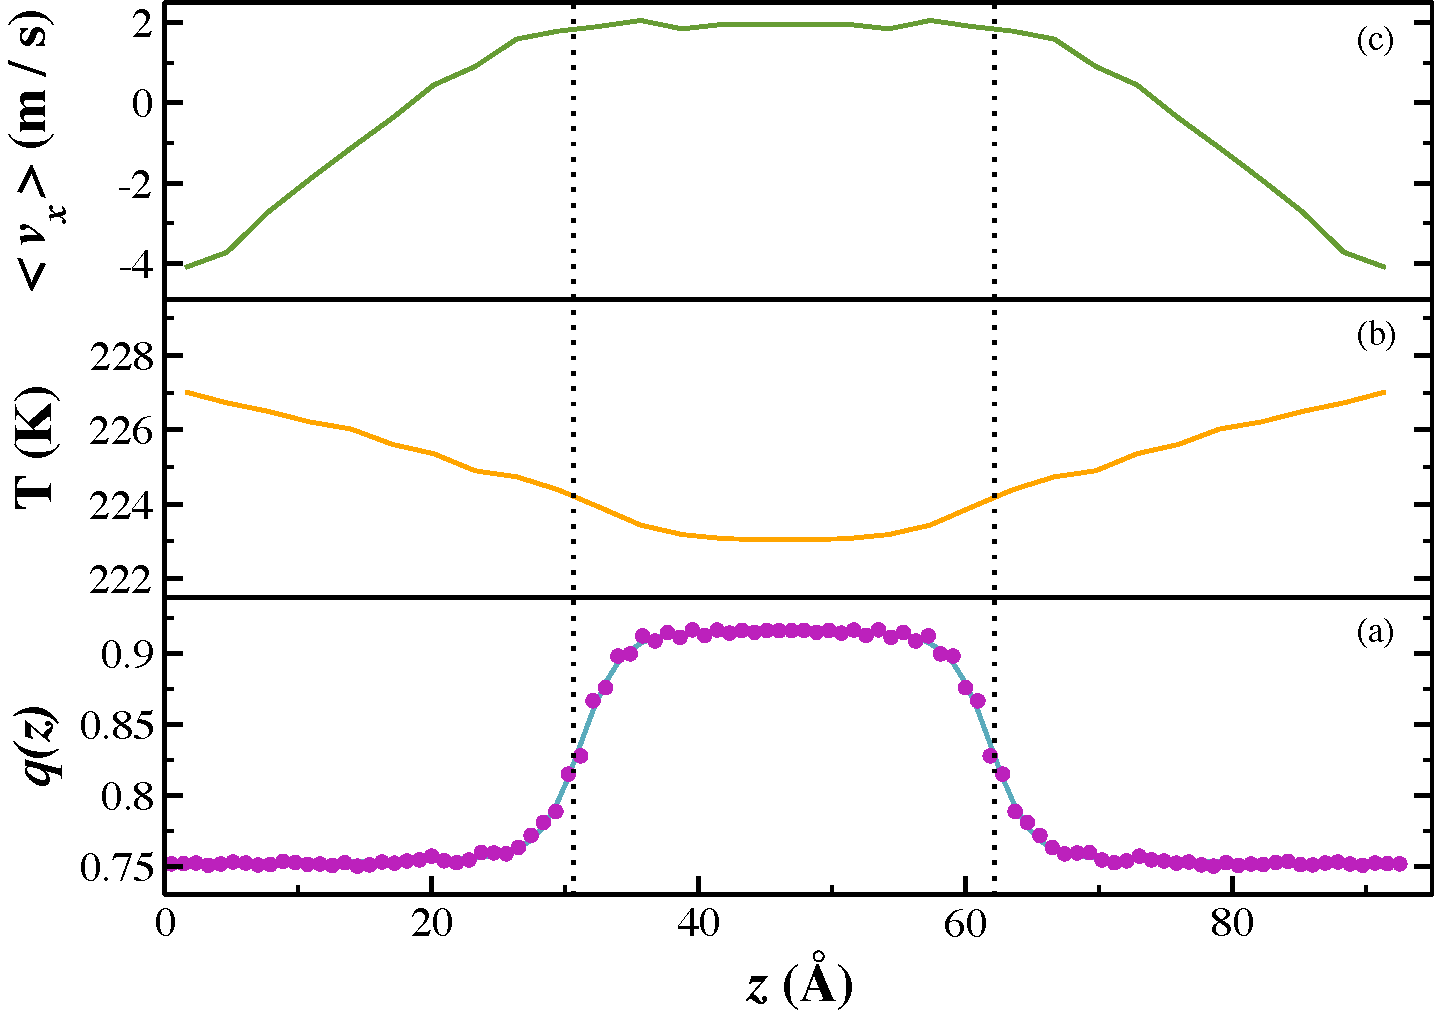
\includegraphics[width=\linewidth]{Pyr_comic_strip}
\caption{\label{fig:pyrComic} The pyramidal interface with a shear
 rate of 3.8 ms\textsuperscript{-1}. Lower panel: the local tetrahedral order
parameter, $q(z)$, (black circles) and the hyperbolic tangent fit (red line).
Middle panel: the imposed thermal gradient required to maintain a fixed
interfacial temperature. Upper panel: the transverse velocity gradient that
develops in response to an imposed momentum flux. The vertical dotted lines
indicate the locations of the midpoints of the two interfaces.}
\end{figure}

\begin{figure}
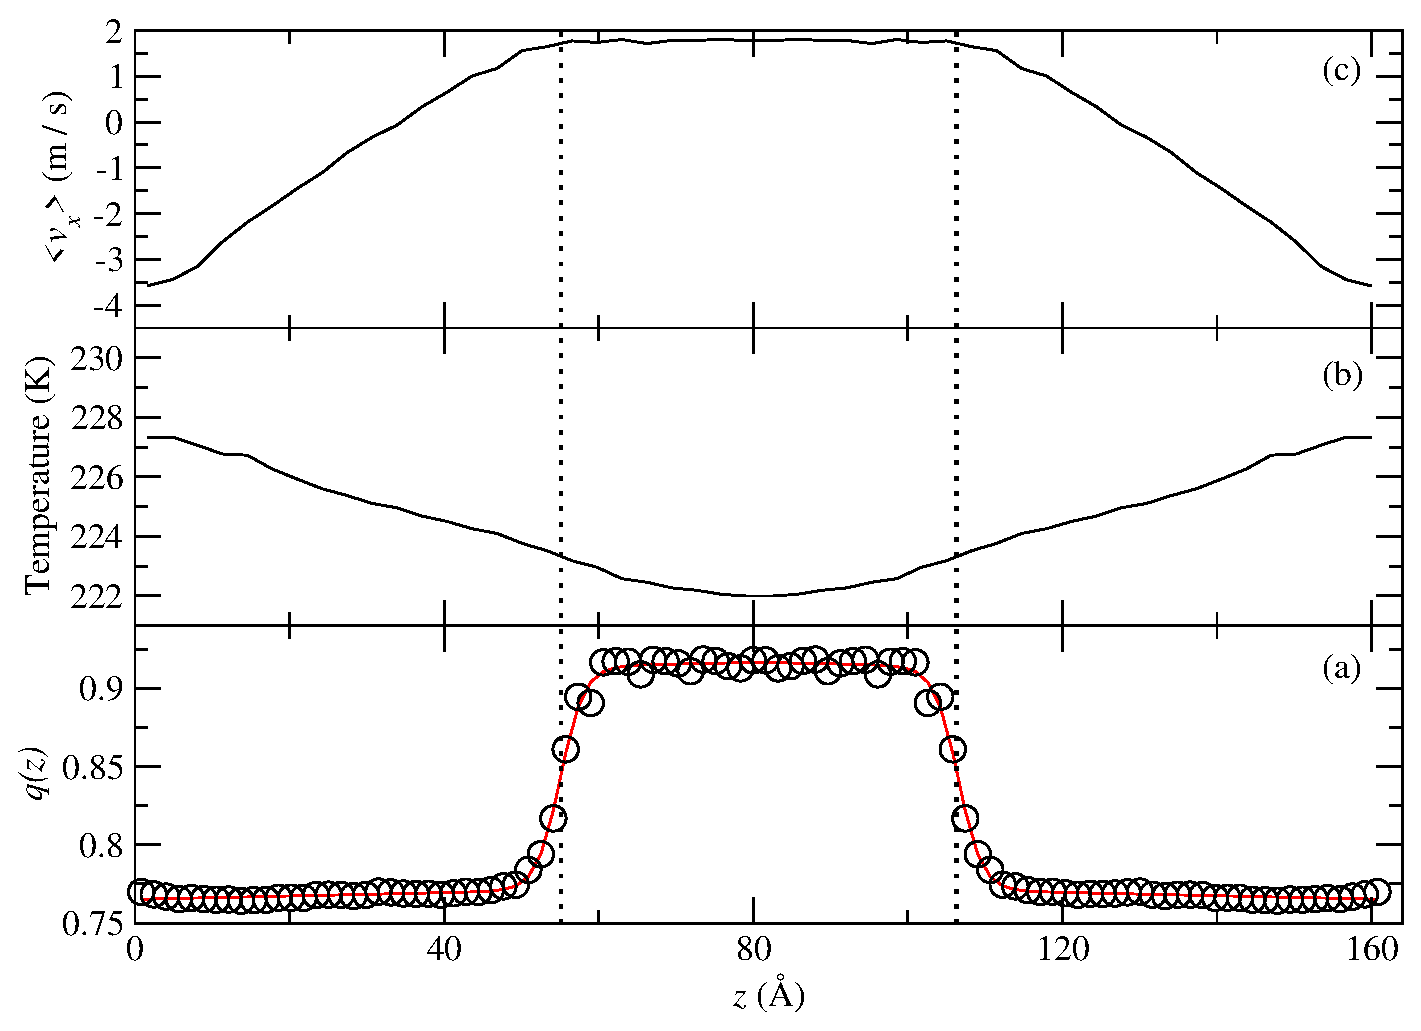
\includegraphics[width=\linewidth]{SP_comic_strip}
\caption{\label{fig:spComic} The secondary prismatic interface with a shear 
rate of 3.5 \
ms\textsuperscript{-1}. Panel descriptions match those in figure \ref{fig:pyrComic}.}
\end{figure}

\begin{figure}
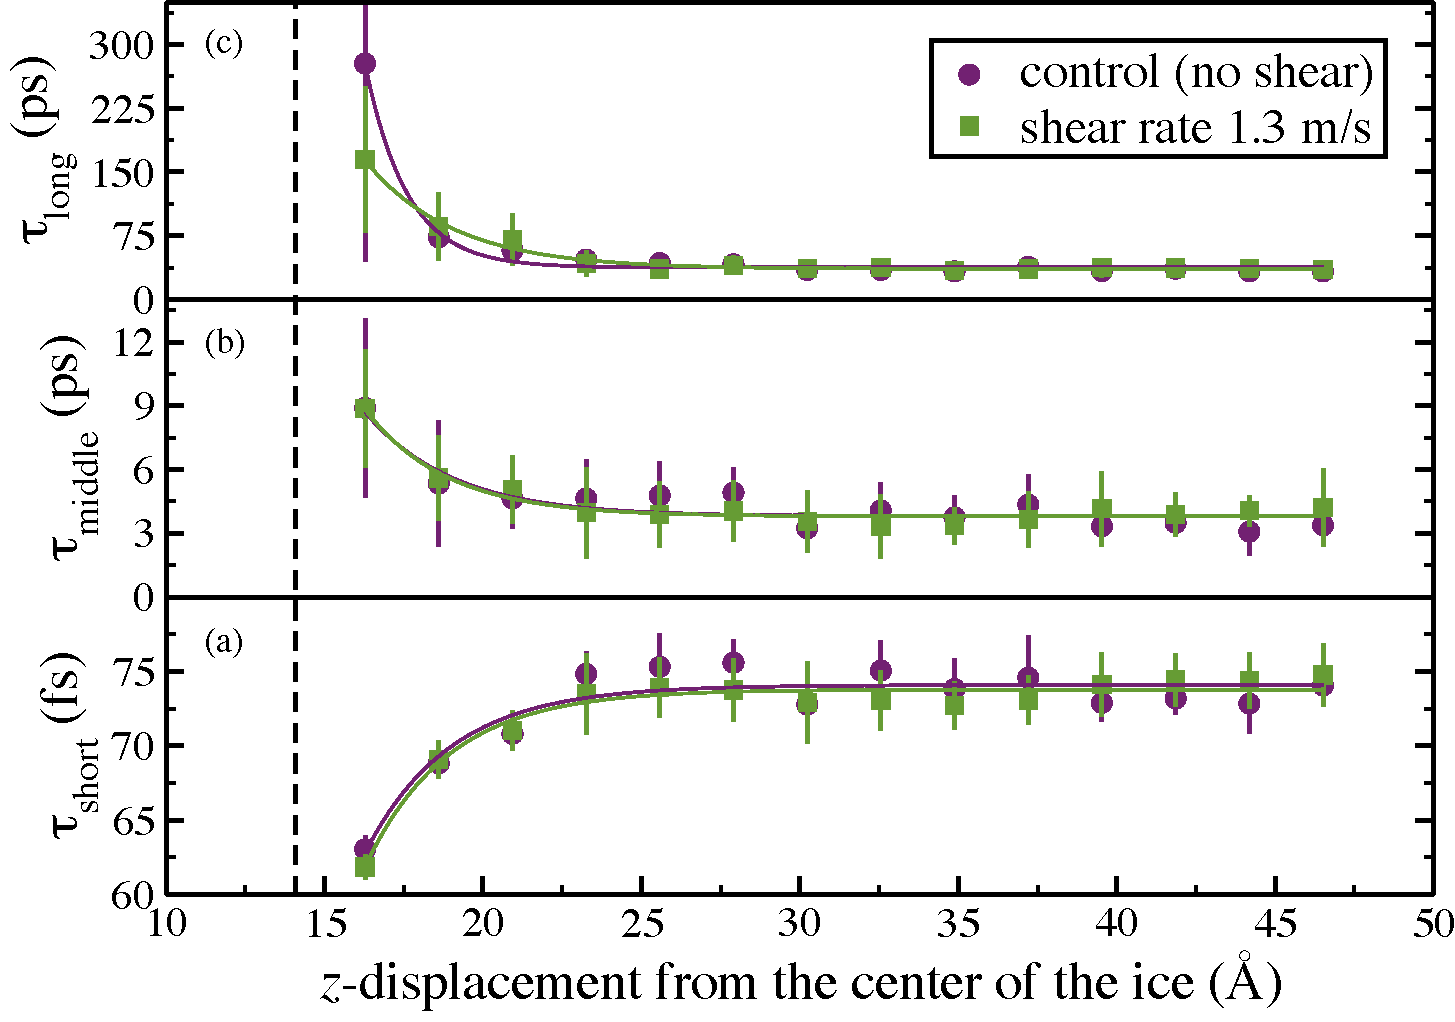
\includegraphics[width=\linewidth]{Pyr-orient}
\caption{\label{fig:PyrOrient} The three decay constants of the 
orientational time correlation function, $C_2(t)$, for water as a function
of distance from the center of the ice slab. The vertical dashed line
indicates the edge of the pyramidal ice slab determined by the local order
tetrahedral parameter. The control (black circles) and sheared (red squares) 
experiments were fit by a shifted exponential decay (Eq. 9\cite{Louden13})
shown by the black and red lines respectively. The upper two panels show that 
translational and hydrogen bond making and breaking events slow down 
through the interface while approaching the ice slab. The bottom most panel
shows the librational motion of the water molecules speeding up approaching
the ice block due to the confined region of space allowed for the molecules
 to move in.}
\end{figure}  

\begin{figure}
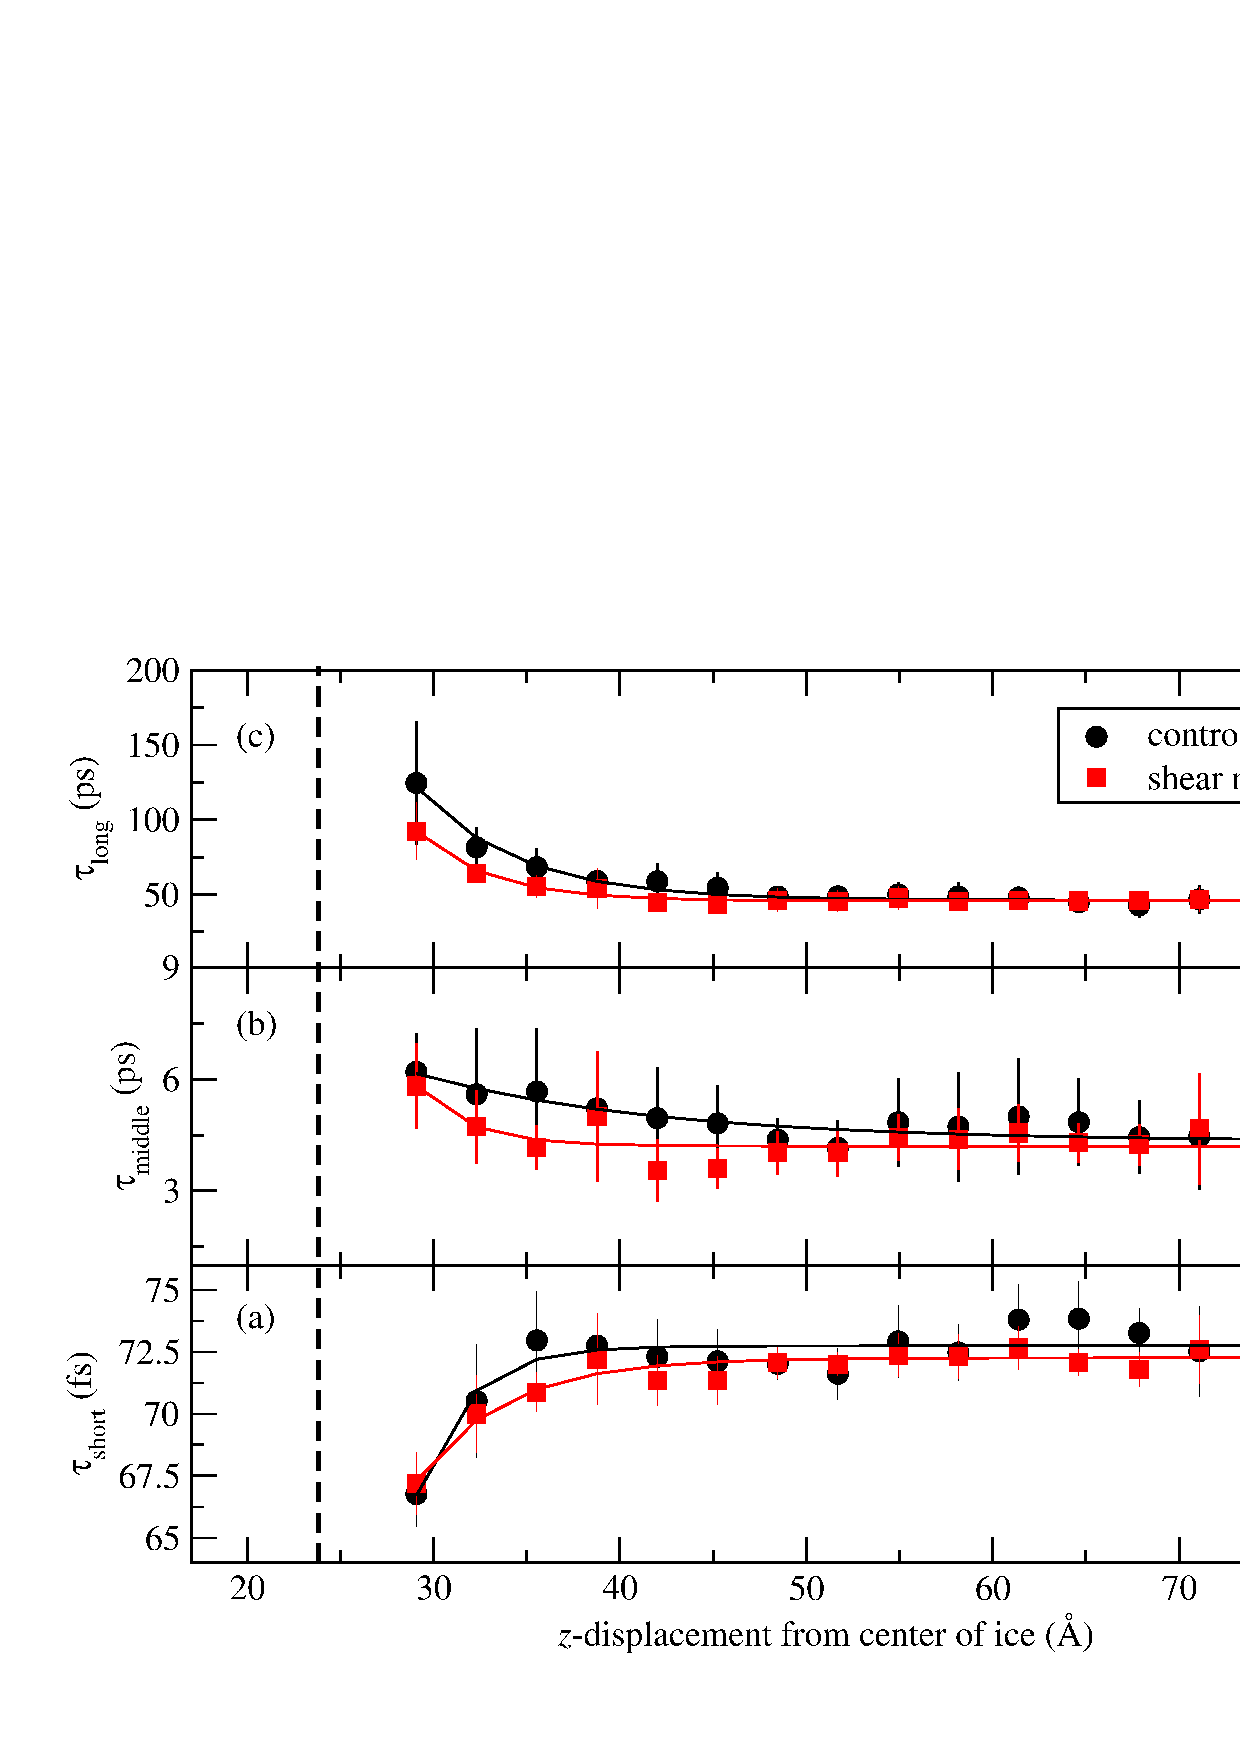
\includegraphics[width=\linewidth]{SP-orient-less}
\caption{\label{fig:SPorient} Decay constants for $C_2(t)$ at the secondary 
prismatic face. Panel descriptions match those in \ref{fig:PyrOrient}.}
\end{figure}


\begin{table}[h]
\centering
\caption{Phyiscal properties of the basal, prismatic, pyramidal, and secondary prismatic facets of Ice-I$_\mathrm{h}$}
\label{tab:kappa}
\begin{tabular}{|ccccc|}  \hline
           & \multicolumn{2}{c}{$\kappa_{Drag direction}$
             (x10\textsuperscript{-4} amu \AA\textsuperscript{-2} fs\textsuperscript{-1})} & & \\
 Interface & $\kappa_{x}$     & $\kappa_{y}$  & $\theta_{\infty}$ & $K_{spread} (ns^{-1})$   \\ \hline
     basal & $5.9 \pm 0.3$ & $6.5 \pm 0.8$ & $34.1 \pm 0.9$ & $0.60 \pm 0.07$  \\
 pyramidal & $5.8 \pm 0.4$ & $6.1 \pm 0.5$ & $35 \pm 3$ & $0.7 \pm 0.1$ \\
 prismatic & $3.0 \pm 0.2$ & $3.0 \pm 0.1$ & $45 \pm 3$ & $0.75 \pm 0.09$ \\
 secondary prismatic & $3.5 \pm 0.1$ & $3.3 \pm 0.2$ & $42 \pm 2$ & $0.69 \pm 0.03$ \\ \hline
\end{tabular}
\end{table}


\begin{table}[h]
\centering
\caption{Shearing and Droplet simulation parameters}
\label{tab:method}
\begin{tabular}{|cccc|ccc|} \hline
& \multicolumn{3}{c}{Shearing} & \multicolumn{3}{c}{Droplet}\\
Interface & $N_{ice}$ & $N_{liquid}$ & Lx, Ly, Lz (\AA) &
$N_{ice}$ & $N_{droplet}$ & Lx, Ly (\AA) \\ \hline
Basal & 900 & 1846 & (23.87, 35.83, 98.64) & 12960 & 2048 & (134.70, 140.04)\\
Prismatic & 3000 & 5464 & (35.95, 35.65, 205.77) & 9900 & 2048 &
(110.04, 115.00)\\
Pyramidal & 1216 & 2203& (37.47, 29.50, 93.02) & 11136 & 2048 &
(143.75, 121.41)\\
Secondary Prismatic & 3840 & 8176 & (71.87, 31.66, 161.55) & 11520 &
2048 & (146.72, 124.48)\\
\hline
\end{tabular}
\end{table}

\end{document}
